\documentclass[10pt]{article}
\usepackage[polish]{babel}
\usepackage[utf8]{inputenc}
\usepackage[T1]{fontenc}
\usepackage{amsmath}
\usepackage{amsfonts}
\usepackage{amssymb}
\usepackage[version=4]{mhchem}
\usepackage{stmaryrd}
\usepackage{graphicx}
\usepackage[export]{adjustbox}
\graphicspath{ {./images/} }

\newcommand\Varangle{\mathop{{<\!\!\!\!\!\text{\small)}}\:}\nolimits}

\begin{document}
\begin{enumerate}
  \item Dany jest równoległobok \(A B C D\) oraz punkt E należący do boku BC. Przez punkt D prowadzimy prostą k równoległą do prostej AE. Na prostej \(k\) obieramy takie punkty K, L, że czworokąt AEKL jest równoległobokiem. Udowodnij, że równoległoboki ABCD i AEKL\\
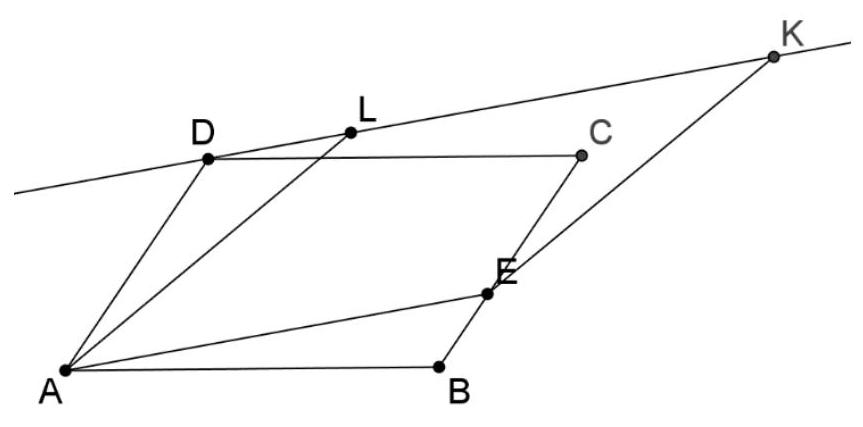
\includegraphics[max width=\textwidth, center]{2024_11_21_5466f38b424164372e40g-1(1)}\\
mają równe pola.
  \item W trójkącie \(A B C\) punkt \(D\) jest środkiem boku AB, a punkt E jest środkiem odcinka CD. Wykaż, że jeżeli \(\Varangle C A E=\Varangle B C D\), to \(A C=C D\).
  \item Powiemy, że liczba całkowita \(n\) jest\\
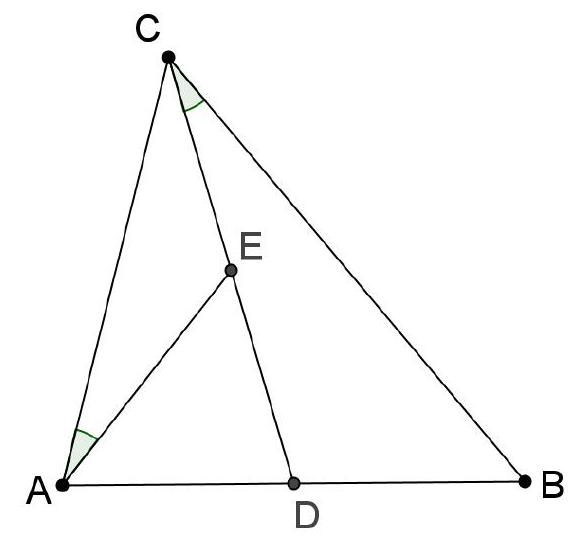
\includegraphics[max width=\textwidth, center]{2024_11_21_5466f38b424164372e40g-1}\\
liczbą śliczną, jeżeli jest sumą kwadratów dwóch liczb całkowitych. Wykaż, że jeżeli \(n\) jest liczbą śliczną, to również 13n jest liczbą śliczną.
\end{enumerate}

\end{document}